
%%%%%%%%%%%%%%%%%%%%%%%%%%%%%%%%%%%%%%%%%%%%%%%%%%%%%%%%%%%%%%%%%%%%%%%%
%    INSTITUTE OF PHYSICS PUBLISHING                                   %
%                                                                      %
%   `Preparing an article for publication in an Institute of Physics   %
%    Publishing journal using LaTeX'                                   %
%                                                                      %
%    LaTeX source code `ioplau2e.tex' used to generate `author         %
%    guidelines', the documentation explaining and demonstrating use   %
%    of the Institute of Physics Publishing LaTeX preprint files       %
%    `iopart.cls, iopart12.clo and iopart10.clo'.                      %
%                                                                      %
%    `ioplau2e.tex' itself uses LaTeX with `iopart.cls'                %
%                                                                      %
%%%%%%%%%%%%%%%%%%%%%%%%%%%%%%%%%%
%
%
% First we have a character check
%
% ! exclamation mark    " double quote  
% # hash                ` opening quote (grave)
% & ampersand           ' closing quote (acute)
% $ dollar              % percent       
% ( open parenthesis    ) close paren.  
% - hyphen              = equals sign
% | vertical bar        ~ tilde         
% @ at sign             _ underscore
% { open curly brace    } close curly   
% [ open square         ] close square bracket
% + plus sign           ; semi-colon    
% * asterisk            : colon
% < open angle bracket  > close angle   
% , comma               . full stop
% ? question mark       / forward slash 
% \ backslash           ^ circumflex
%
% ABCDEFGHIJKLMNOPQRSTUVWXYZ 
% abcdefghijklmnopqrstuvwxyz 
% 1234567890
%
%%%%%%%%%%%%%%%%%%%%%%%%%%%%%%%%%%%%%%%%%%%%%%%%%%%%%%%%%%%%%%%%%%%
%
%%novalidate

\documentclass[12pt,a4paper,final]{iopart}
\newcommand{\gguide}{{\it Preparing graphics for IOP journals}}
%Uncomment next line if AMS fonts required
\usepackage{iopams}
\usepackage{graphicx}
\usepackage[breaklinks=true,colorlinks=true,linkcolor=blue,urlcolor=blue,citecolor=blue]{hyperref}

% Custom for this paper
\bibliographystyle{iopart-num}
%\usepackage{amsmath,amssymb,amsfonts}
%\usepackage{mathtools}
% for \code color
\usepackage[dvipsnames]{xcolor}
\usepackage{todonotes}
\usepackage{menukeys}
\usepackage{siunitx}
\usepackage{listings}
% Pretty formating of c++ (see \cpp command)
\usepackage{xspace}
\newcommand*{\cpp}{C\ensuremath{++}\xspace}

\lstdefinelanguage{LAMMPS}{
	morekeywords={units,compute,langevin,atom_style,lattice,region,create_box,create_atoms,pair_style,pair_coeff,neigh_modify,mass,velocity,fix,run, group every, equal, count, porosity, EDGE},
	sensitive=false, % keywords are not case-sensitive
	morecomment=[l]{//}, % l is for line comment
	morecomment=[s]{/*}{*/}, % s is for start and end delimiter
	morestring=[b]" % defines that strings are enclosed in double quotes
}

\lstset{
basicstyle=\small,
frame = single,
language=LAMMPS,
framexleftmargin=15pt,
xleftmargin=0.65cm,
xrightmargin=0.1cm}

% Highlighte inline code
\definecolor{light-gray}{gray}{0.95}
\definecolor{atomify-red}{rgb}{0.90196078 , 0.09803922, 0.29411765}
\definecolor{atomify-green}{rgb}{0.23529412 , 0.70588235, 0.29411765}
\definecolor{atomify-yellow}{rgb}{0.8,  0.70588235,  0.07843138}
\definecolor{atomify-blue}{rgb}{0.00000000 , 0.50980392, 0.78431373}
%\newcommand{\code}[1]{\mbox {\texttt{#1}}}
\newcommand{\code}[1]{\colorbox{light-gray}{\color{RawSienna}\texttt{#1}}}

\begin{document}

\title{Effective workflow in molecular dynamics simulations using Atomify --- a real-time LAMMPS visualizer}

\author[cor1]{Anders Hafreager$^{1}$}
\eads{\mailto{anderhaf@fys.uio.no}, \mailto{andershaf@gmail.com}}

\author{Svenn-Arne Dragly$^{1}$}
\ead{s.a.dragly@fys.uio.no}

\author{Anders Malthe-S\o renssen$^{1}$}
\ead{malthe@fys.uio.no}
\address{$^1$Department of Physics - University of Oslo\\Sem S{\ae}lands vei 24, NO-0316, Oslo, Norway}

\begin{abstract}
A typical workflow when setting up and running atomistic simulations combines the use of several tools:
a text editor to create and modify scripts; the terminal to run the simulation; and programs like VMD or Ovito to visualize the dynamics of the system. In addition, to study the behavior of physical quantities, relevant data must be computed, stored, and subsequently plotted. This is a cumbersome process, which limits the use of atomic simulation tools for teaching and increases the barrier of adaptation for newcomers. 
Here, we introduce Atomify to streamline the atomic simulation workflow. It is a user-friendly high-performance real-time visualizer for atomistic simulations that can simulate and render more than one million atoms with excellent frame rate on modern hardware.
Atomify supports OpenMP acceleration, GPU acceleration, real-time plotting of physical quantities, and an easy-to-use code editor in one single application.
It currently uses LAMMPS as physics engine, but it can be extended to support other underlying codes like GROMACS, NAMD or CHARMM.
Atomify is open-source software (GPL) written in C++ using the Qt framework and can be downloaded from \url{https://github.com/ovilab/atomify}.
\end{abstract}

%Uncomment for PACS numbers title message
% \pacs{00.00, 20.00, 42.10}
% Keywords required only for MST, PB, PMB, PM, JOA, JOB? 
\vspace{2pc}
% Comment out if separate title page not required
%\maketitle

\section{Introduction}
Atomic scale simulations using molecular dynamics simulations have become a standard tool in scientific research, development and education\cite{frenkel2001understanding,StatisticalAndThermalPhysics-Gould-2006}.
However, the workflow to set up and run molecular dynamics simulations has remained mostly unchanged over the past decades.
Users of LAMMPS\cite{Plimpton1995Fast}, GROMACS\cite{berendsen1995gromacs}, NAMD\cite{nelson1996namd} and CHARMM\cite{brooks2009charmm} typically write
scripts in a text editor, run the scripts by passing them to the simulator on the command line. 
The simulator in turn writes the results to disk, and the user then analyzes the results
by reading the files manually or passing them to other programs.

With the introduction of software like Rasmol\cite{sayle1995rasmol} and VMD\cite{Humphrey1996Vmd},
it became easy to both visualize simulation trajectories and analyze calculated quantities such as the radial distribution function within the same tool. 
VMD came with support both for reading trajectories from file and attaching to a
running process using MDComm\cite{nelson1995mdscope} and a supported simulator such as NAMD.

Some 10 years later, an improved abstract communication layer called MDDriver\cite{delalande2009complex} was designed.
Compared to MDComm it was more general and required only a small effort to add support for a new simulator. Another visualization tool MegaMol\cite{grottel2015megamol} was developed more recently and supported real-time visualization of GROMACS through MDDriver.
However, data was transferred through the IMD protocol based on TCP/IP sockets\cite{delalande2009complex}, and this may have introduced
overhead in the data transfer compared to a shared memory solution.
Although this enabled real-time visualizations, the workflow was not very user-friendly since it still involved
the use of different programs that all needed to be configured a particular way.

Analysis of simulations is often done as a postprocessing step where the trajectories and other 
per-atom quantities, such as velocity and stress, are loaded into an analysis tool often written by researchers themselves.
One of today's most popular visualization tools for atomistic simulations is OVITO\cite{Stukowski2009Visualization},
which introduced a powerful modifier pipeline where input data can be processed and manipulated as a series of scriptable building blocks.
These building blocks can be used to calculate new properties, and atoms can be colored accordingly.

In addition, aggregate scalar quantities such as temperature, pressure or number of atoms in a specific state are often stored to a
text file. Researchers then write their own plotting scripts in languages like MATLAB or Python
to plot the time evolution of these quantities. 

In combination, the text editors, the simulators, the visualization software, and MATLAB or Python scripts define the workflow of a typical researcher in computational
materials science.
While this is a powerful workflow in well-established simulation cases,
it is tedious for prototyping new ideas.
This workflow requires a fairly large amount of context switching,
moving from the text editor to the terminal to run the simulation,
waiting for the results, and then finally being able to study them using the analysis
and visualization tools.

Here, we present Atomify, a software that integrates script editing,
visualization and analysis into one tool.
Atomify uses LAMMPS as a linked library and has shared memory access to the internals of LAMMPS,
which maximizes the data transfer speed and reduces latency.
By having direct access to all the data structures in LAMMPS, Atomify is capable of not only visualizing the simulation results,
but also show additional information about how the simulation is defined using groups and regions.

This is especially useful during development of new scripts, but can also be used
to run full, publication-ready simulations with minimal simulation overhead.
The current implementation only supports LAMMPS as a simulator, but it is written in a general
way so integrating other codes is a simple task.

\begin{figure}
	\centering
	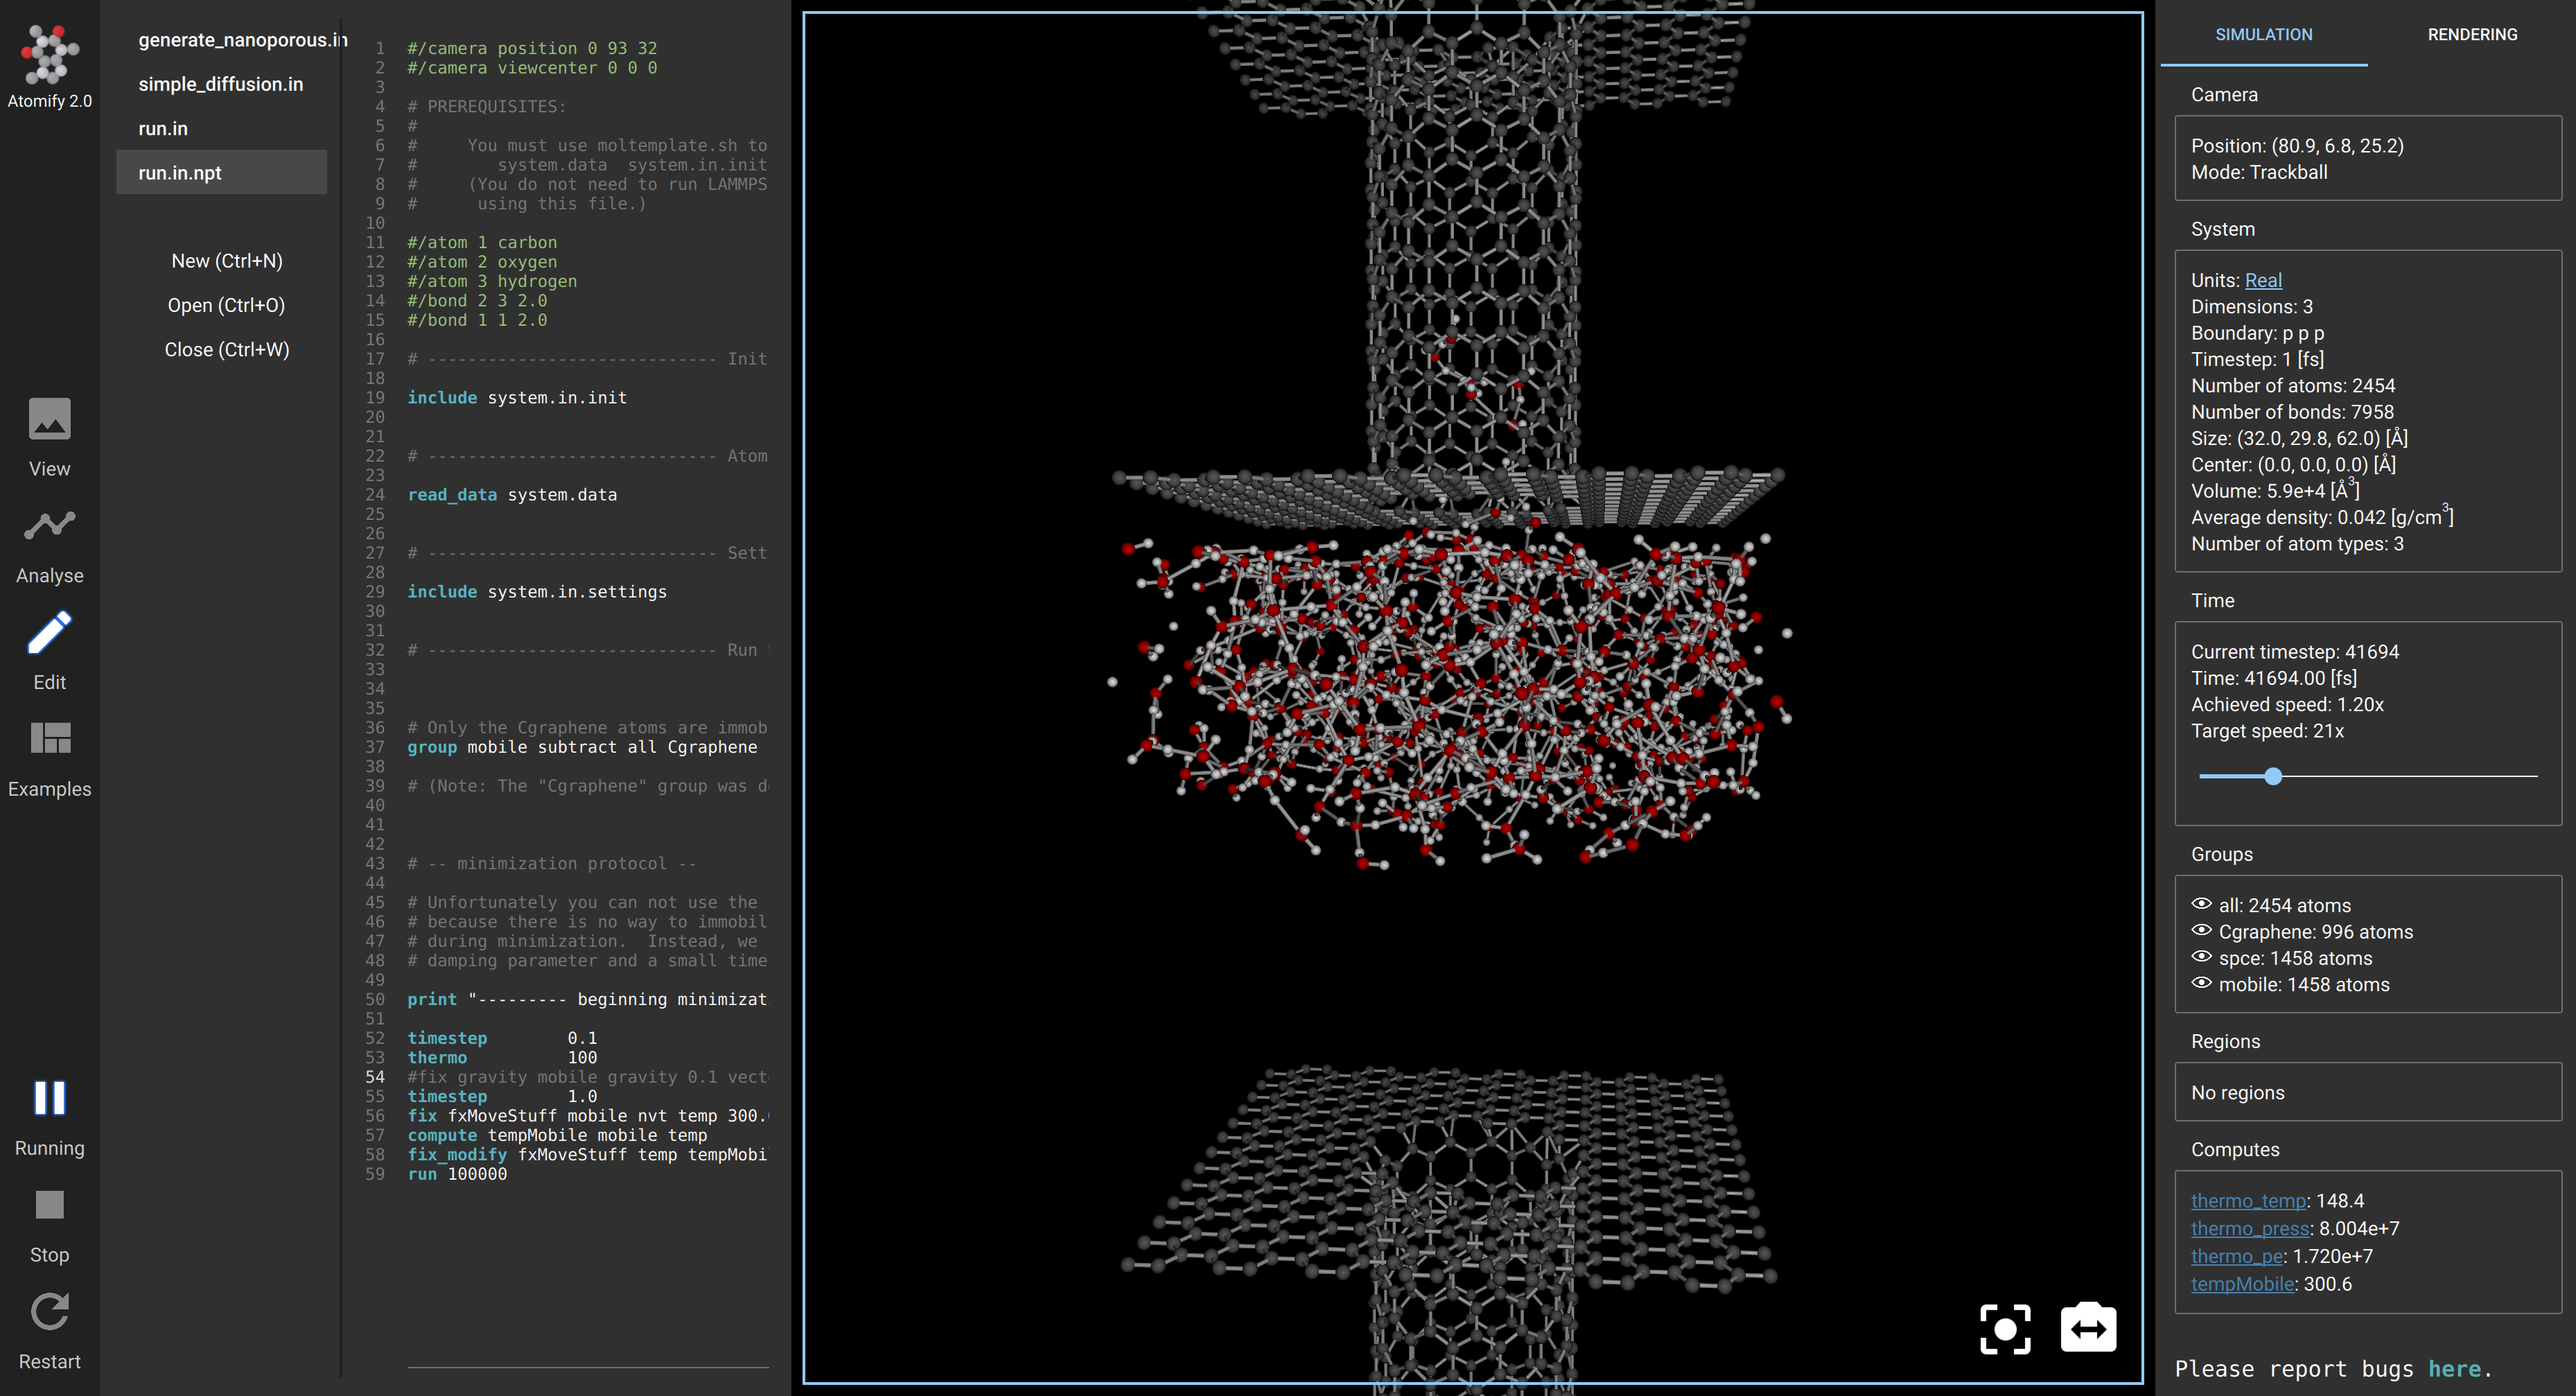
\includegraphics[width=\textwidth]{figures/gui.pdf}
	\caption{%
	Overview of the Graphical User Interface (GUI) in Atomify.
	The toolbar a) is used to change between the different modes, such as
	editing, viewing and analyzing the running simulation.
	The bottom of a) contains the playback controls.
	The script editor b) supports multiple open files and provides simple syntax highlighting.
	The viewport c) shows the current simulation with atoms and bonds, simulation box and coordinate axes.
	The simulation properties d) shows the simulations details, presents
	LAMMPS objects such as groups, regions, computes, variables and fixes, and the rendering
	properties. If one of the computes, variables or fixes with plottable data is clicked, a plot window
	e) is shown with simple plot properties and export functions to MATLAB, Python or a text file.
	}
	\label{fig:gui}
\end{figure}

In this paper we will 
introduce and demonstrate many of the useful features that Atomify provides through a case study. 
We start by introducing the GUI in section \ref{sec:features}, which also summarizes the main features of Atomify.
In section \ref{sec:casestudy}, the case study is introduced. Here, we provide a detailed walk-through of setting up, running and analyzing a non-trivial simluation that uses regions and groups to perform different integration rules on different atoms.

\begin{figure}[htp!]
	\centering
	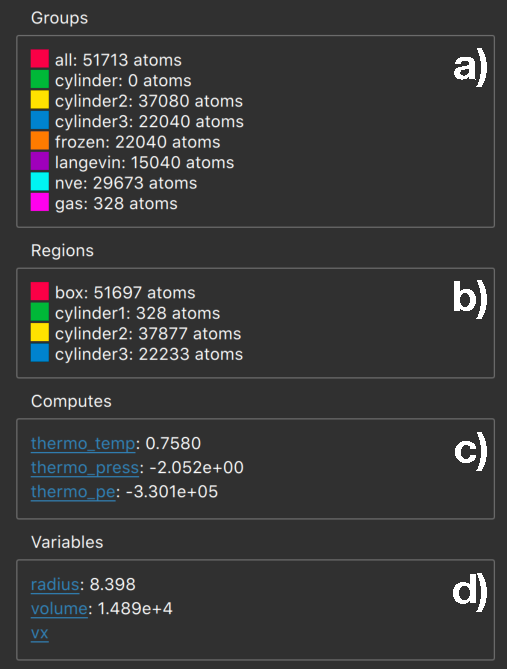
\includegraphics[width=0.5\textwidth]{figures/rightbar.pdf}
	\caption{
		The \textit{Simulation} panel is a powerful feature in Atomify where relevant
		properties from LAMMPS are presented real-time.
		In a), a list of all defined groups is shown with the current atom count.
		b) shows all defined regions. Each group and region can be hovered with the mouse so that atoms
		are colored after what group/region they are in. If an atom is in multiple
		groups or regions, they will get the color of the latest one defined.
		The color boxes can be clicked to either always highlight the atoms in a certain group or region,
		or if clicked again, hide all of them.
		In c) and d), a list of all variables and computes is shown. If a variable or a compute
		produce a scalar, the current value is shown as can be seen with all the variables.
		By clicking the name, a plot will show up with the time evolution of that quantity.
		If a per-atom variable or compute is hovered, all atoms will be colored according to their
		current scalar value and a histogram over these values is shown if clicked.
		The result of hovering atoms defined by the groups in our case study is shown in figure \ref{fig:cylinder_simulation}.
	}
	\label{fig:rightbar}
\end{figure}

\section{\label{sec:features}Summary of features}
The Atomify graphical user interface (GUI) is shown in figure \ref{fig:gui}.

Atomify was designed with one goal at mind: to improve the workflow.
By focusing on minimizing the number of context switches and mouse clicks, 
the distance between creativity and simulation results is reduced. 
Atomify has a script editor, a visualization window and a simulation summary panel enabling all relevant parts
of a simulation to be on the screen at the same time.

The effect of any changes to the script, such as defining regions or groups,
changing temperatures or the size of the simulation box, or inserting atoms, can
quickly be checked since the visualization shows the real-time state of the simulator.
Rerunning the current script can be done by pressing \keys{Ctrl+R} (\keys{\cmd+R} on macOS).

The temporal evolution of the pressure, the radial distribution function or any other
variable can be plotted real-time with a simple click in the list of variables.
Bonds between atoms in a molecule are automatically extracted from LAMMPS, or can
be specified as a distance threshold between atom types.
Regions and groups can be highlighted or hidden, which is useful to focus on some parts of a system.
Rendering of periodic copies helps studying features near a periodic boundary.

When the simulation produces per-atom scalar quantities, Atomify can color each atom based the value.
For instance, \code{compute cna/atom}\cite{faken1994systematic, tsuzuki2007structural} can be used to identify the crystal structure an atom is a part of.
It gives each atom an integer value in the range [1,5] representing FCC, HCP, BCC, Icosohedral or unknown crystal structure.
\code{compute displace/atom} can be used to see how far each atom has moved and \code{compute stress/atom} gives the local stress in the system.
More complicated variables using per-atom data can be defined with the general scripting language in LAMMPS.
If desired, these values can be time averaged using \code{fix ave/atom} and used to color each atom according to the value.

Although LAMMPS is mostly used to study molecular dynamics, it can also be used to
model Monte Carlo simulations\cite{frenkel2001understanding} and granular
materials\cite{brilliantov1996model, silbert2001granular, zhang2005jamming},
both of which work in Atomify since they are particle based simulations.

Atomify supports rendering of spheres and cylinders to represent atoms and bonds.
It is done using Qt3D with custom visualization techniques such as
billboard raycasting\cite{gumhold2003splatting, sigg2006gpu, tarini2006ambient} and screen space ambient occlusion\cite{bavoil2008screen}
for improved dynamic depth perception. This allows a large amount of atoms and molecules to be rendered with excellent framerate.
The liming factor is the simulation itself, since force calculation is a computationally intensive task.

In addition, Atomify comes with substantial database of examples,
many of which have been made by members of the LAMMPS community.

\section{\label{sec:casestudy}Case study: flow through a narrow nanotube}
Atomify is best demonstrated through a case study that shows how 
various features can be used in a productive workflow from script development to analysis.
We have chosen to address fluid flow inside a narrow, cylindrical nanochannel, since this is a scenario that demonstrates many of the features of Atomify and its integrated workflow: The simulation involves creating an initial geometry with multiple regions 
where we apply different rules such as a dissipative thermostat, a constant force mimicking
an applied pressure gradient, and frozen atoms to avoid net momentum of the solid.
We introduce two different atom types in order to have a gas phase and a solid phase at the same temperature.

Fluid flow in porous structures is often characterized by its permeability, $k$, which describes the fluid flow conductivity of a fluid in a specific geometry. Darcy's law relates the average flow velocity, $U$, to the applied pressure gradient $\nabla P$: $U = (k/\mu)(-\nabla P)$, where $\mu$ is the viscosity of the fluid. In Darcy's law, the permeability is assumed to only depend on the material and its geometry. 
\todo[inline]{U is the flux here, not the average velocity?}
However, Darcy's law must be modified for dilute
gases where the measured permeability also is found to also be a function of pressure.
This is called the Klinkenberg effect\cite{klinkenberg1941permeability}.

The discrepancy is due to finite slip of the dilute gas along the pore walls. For a macroscopic fluid, the velocity of the fluid is usually assumed to be zero at the pore walls. This is called non-slip boundary conditions and is a good approximation for dense liquids in macroscopic pores. However, if the typical channel size $R$ in the pores is of the same order as the mean free path $\lambda$ of the fluid, non-slip boundary conditions are no longer a good approximation to the actual flow profile. The ratio between the mean free path and the channel size is quantified through
the Knudsen number, $\text{Kn} = \lambda / R$ is used in the Klinkenberg correction\cite{klinkenberg1941permeability} for the \textit{effective permeability} as a function of pressure in the limit of high Knudsen numbers. Such a system is well suited for a molecular dynamics study because channles with small values of $R$, and hence high Knudsen numbers, may be studied in molecular systems.

\begin{figure}
	\centering
	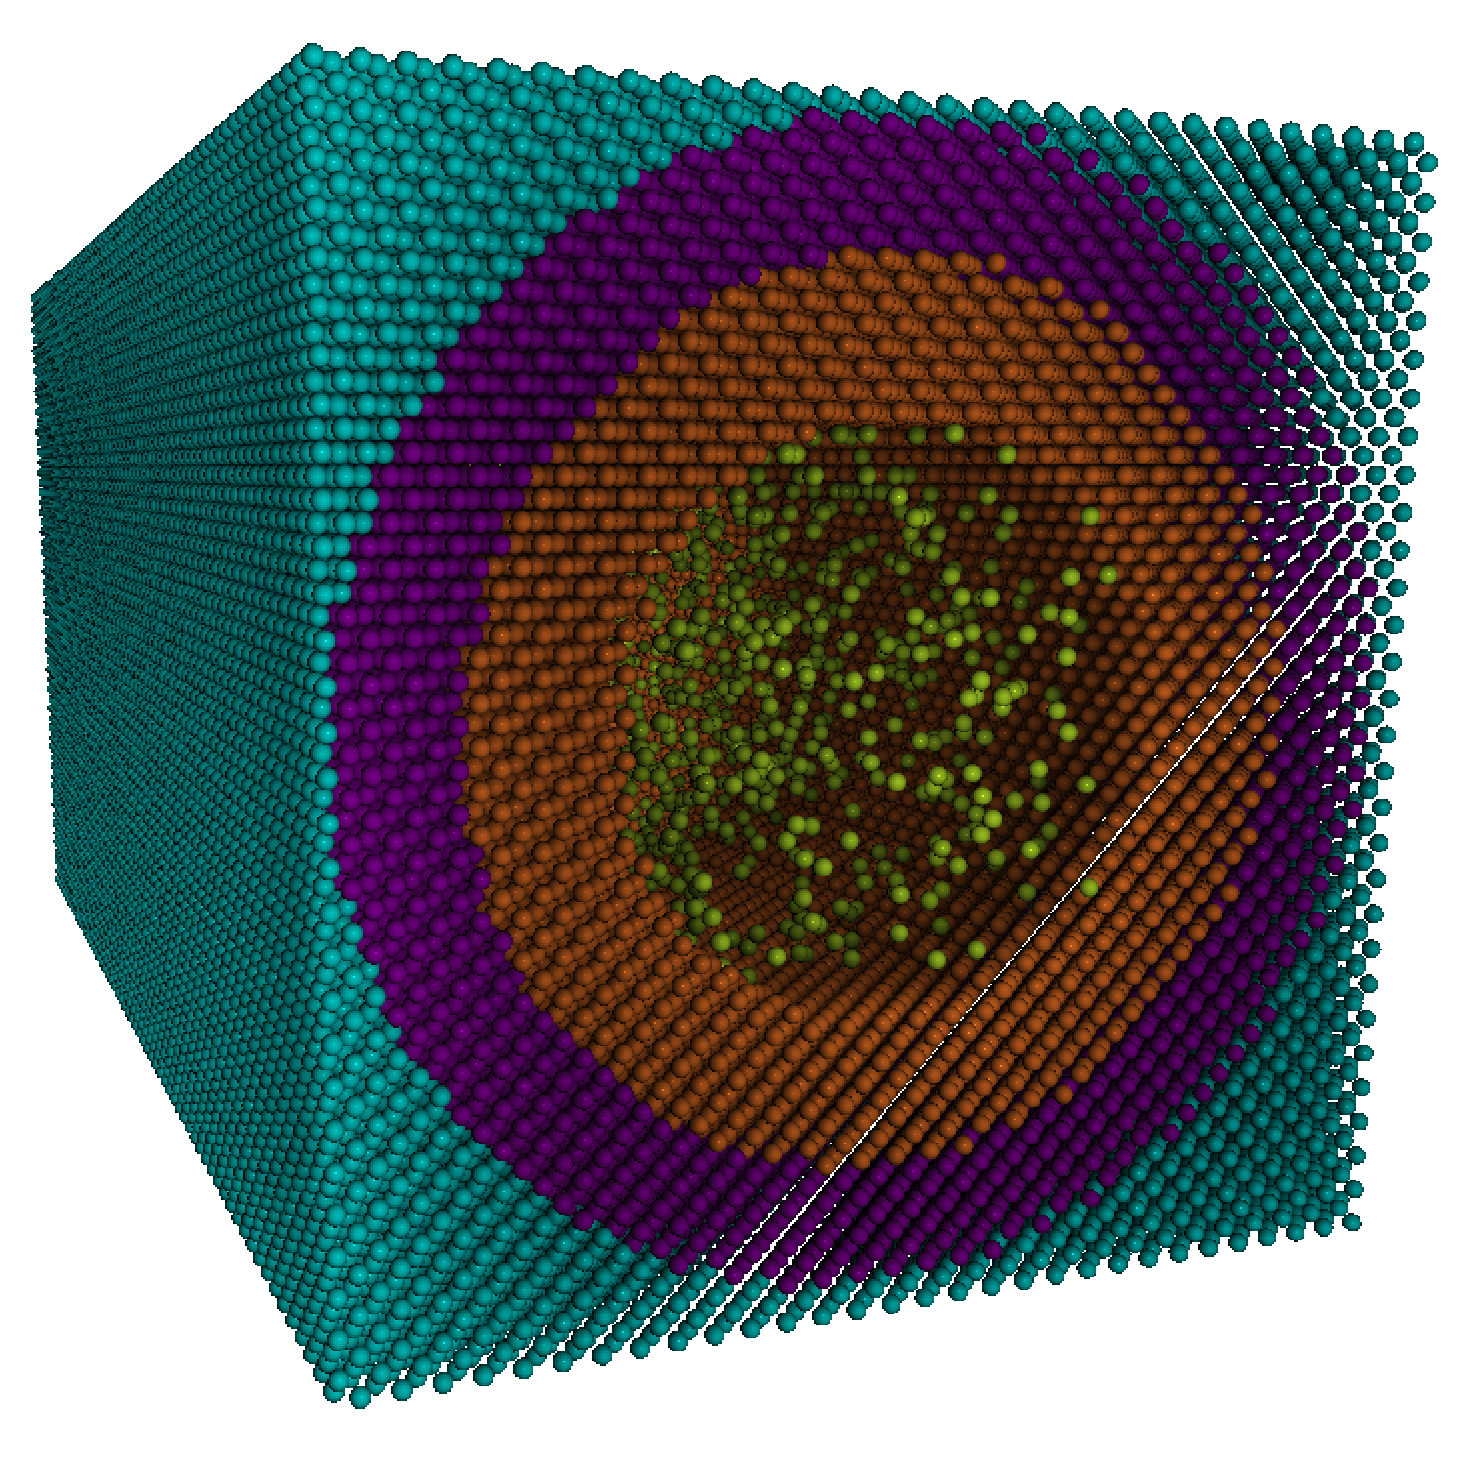
\includegraphics[width=0.75\textwidth]{lj_flow/configuration.png}
	\caption{
		Initial configuration in our case study simulation.
		A periodic box consisting of $(60\times30\times30)$ FCC unit cells with reduced density $\rho^* = 0.975$ where we will have gas flow in a cylinder with radius 12.
		The different colors indicate the regions of which different integration rules apply.
		Cyan atoms are fixed and do not move at all,
		whereas the purple atoms are thermalized with a Langevin\cite{schneider1978molecular} dissipative thermostat to mimick the heat exchange with the frozen bulk atoms.
		The orange and the yellow atoms are integrated normally, but the yellow gas atoms also have an applied constant acceleration representing the pressure gradient.
		Setting up and verifying the system is simple using Atomify due to i.e. the real-time coloring of groups and regions.
	}
	\label{fig:cylinder_simulation}
\end{figure}

\subsection{Physical description of the simulation system}
In this case study, we will use Atomify to measure the velocity profile of a
gas inside a nanotube with varying density to directly observe
the slip velocity at low densities.
We will use the Lennard-Jones potential with two different atom types.

We create a nanotube inside a FCC solid with $(60\times30\times30)$ unit cells and reduced density $\rho^* = 0.975$.
The density was chosen to ensure that the two atom types with the Lennard-Jones coefficients specified below will coexist in different phases. We will apply a pressure gradient to the fluid inside the nanotube to induce fluid flow, see figure \ref{fig:cylinder_simulation}.
We apply a pressure gradient $\nabla P$ in the $x$-direction on the gas atoms using an added force, which corresponds to an acceleration $a$ added to each atoms. The acceleration $a$ calculated as
\[
	a = \frac{\nabla P}{\rho_m},
\]
where $\rho_m$ is the mass density of the gas atoms, produces the desired pressure gradient $\nabla P$.
This represents a pressure difference $\Delta P$ over a small volume element $\Delta x$ on a cross-sectional area $\Delta y\Delta z$.

By adding an external force to atoms in the system, energy is added to the system, which in turn will increase the temperature and eventually melt the system or make it move.
To avoid this, we couple the solid to an external heat bath so the added energy can be transferred out from the system through a dissipative thermostat.

Even though we only apply a pressure gradient on the gas atoms, the induced momentum will also be transferred
to the solid atoms, which eventually will start moving in the positive $x$-direction.
We want the solid to be at rest, since only the relative velocity between the gas and the solid defines
the flow. We will therefore freeze the outermost atoms (colored cyan in Fig \ref{fig:cylinder_simulation}).

To obtain this system, we divide the atoms into multiple cylindrical regions, which are integrated differently:

\begin{itemize}
	\item $r \leq 12$: gas atoms with applied pressure gradient
	\item $18 < r \leq 21$: dissipative Langevin thermostat
	\item $21 < r$: frozen.
\end{itemize}

The different radii are specified in reduced Lennard-Jones units.

In the following we will provide a detailed description of how to set up, run and analyze this system using Atomify.

\subsection{Creating the initial geometry}
We create a new script in Atomify using \keys{Ctrl+N}, and save it with \keys{Ctrl+S} as \code{run.in}.
Copy the following input script

\lstinputlisting[language=LAMMPS]{simple.in}

We will modify and adapt this script to bit by bit to correspond to the system we want to simulate.
Here, we have a Lennard-Jones solid with reduced density
$\rho^* = 0.975$, reduced masses $m_1^* = 4.0$, $m_2^* = 0.5$ with $(60\times30\times30)$
FCC unit cells and a cutoff of $2.5$. 
The force field parameters are chosen so that atoms of type 1
are in the solid phase while type 2 atoms are gas at reduced temperature $T^*=0.5$.
The two atom types are weakly coupled (small $\epsilon_{ij}$) so the gas atoms won't
stick too easily to the surface since this would prevent flow.

To make sure LAMMPS executes our modification before visualization is started,
we need to make sure that following additional commands happen \textit{before} the \code{run 1000} command.
If not, LAMMPS will run 1000 timesteps before getting to our changes.

To define the inner cylinder, we first specify the radius and the center before using the region command
\begin{lstlisting}
variable R equal 12
variable c equal $(ly*0.5)
region cylinder1 cylinder x $c $c $R EDGE EDGE
set region cylinder1 type 2
\end{lstlisting}
The region command will create a cylinder $C_1$ in the $x$-direction, with $(y,z)$-coordinates at the 
system center \code{\$c} with radius \code{\$R} using the full length of the system in the $x$-direction specified with \code{EDGE}.
We also change the atoms inside the region to type 2 since these are the gas atoms.

We now press \keys{Ctrl+R} to run the simulation to see how it looks.
As shown in figure \ref{fig:rightbar}, we can hover the specified region to highlight the atoms in it.

\begin{figure}
	\centering
	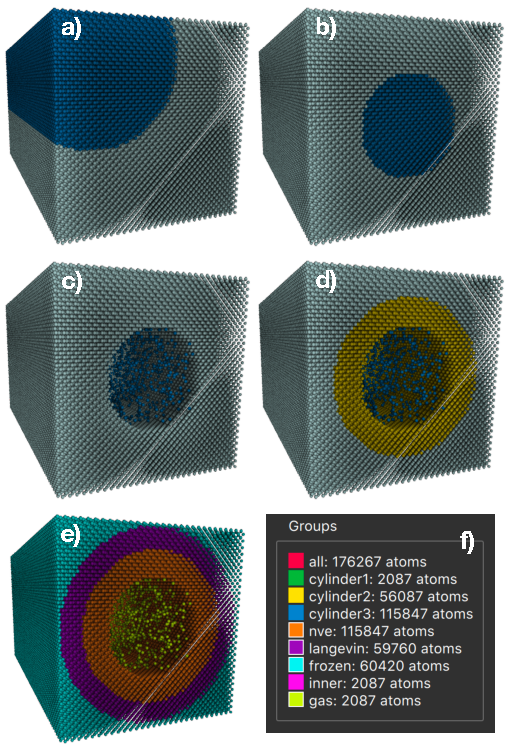
\includegraphics[width=0.8\textwidth]{figures/initial_configuration.pdf}
	\caption{
		Several snapshots of the process of creating the simulation in our case study.
		This shows how one typically generates a geometry step by step where the immediate
		feedback is very useful to quickly discover mistakes.
		The wrongly placed cylinder is shown in a) whereas it is placed correctly in b).
		c) shows how the system looks after deleting atoms to obtain $\rho_m = 0.05$. The next cylinder $C_2$ is shown in d),
		and all regions (placed in groups) are shown in e). Here we have uniquely defined the purple shell which should have a dissipative thermostat.
		In f), the list of all groups defined in this system is shown with colors matching those of e).
		Although one group is colored green, we don't see any green atoms (\code{cylinder1})
		since all of them also are in the groups \code{cylinder2}, \code{cylinder3}, \code{nve} and \code{gas},
		which all override the color. The color of an atom is determined by the last defined group it is a member of.
		All figures are rendered with Atomify.
	}
	\label{fig:initial_configuration}
\end{figure}

When we hover the region, we immediately see that the cylinder is not placed at the center of the system, as shown in figure \ref{fig:initial_configuration}a.
The reason is that LAMMPS operates with two different units, either the length unit or the lattice length unit. This is explained in the documentation, but is a common mistake.
Discovering mistakes like this is easy using Atomify.

Since we used \code{\$(0.5*lx)}, which gives the system length in actual lenght units, we need to specify \code{units box} in the region command:
\begin{lstlisting}
	region cylinder1 cylinder x $c $c $R EDGE EDGE units box
\end{lstlisting}
We then rerun the simulation with \keys{Ctrl+R} and see that we get the wanted result in figure \ref{fig:initial_configuration}b.

Now that the region looks right, we want to delete some atoms to control the density.
The volume of the inner cylinder is $\pi R^2 L$ which can be calculated in LAMMPS with \code{variable V equal PI*v\_R*v\_R*lx}.
The command \code{delete\_atoms} can be used: \code{delete\_atoms porosity region-ID fraction seed},
where we need to specify what fraction of the existing atoms in the region that we want to delete, and a random seed which can be any positive number.
Since we want to specify a specific density, we need to figure out how many atoms we
should delete. This depends on the current number of atoms inside the region.

To count the number of atoms inside a region, we first create a group containing all the atoms in it, and then create a variable that counts them.
Assuming mass density $\rho_m = 0.05$, we can calculate the expected number inside the cylinder as $N = V\rho_m/m$,
where $V$ is the volume of the cylinder and $m$ is the mass of type 2 atoms.

The atoms inside the region can now be deleted with the following commands
\begin{lstlisting}
group cylinder1 region cylinder1
variable N_cyl equal count(cylinder1)
variable V equal PI*$R*$R*lx
variable rho_m equal 0.05
variable N_wanted equal $V*${rho_m}/0.5
variable delete_fraction equal (${N_cyl}-${N_wanted})/${N_cyl}
delete_atoms porosity cylinder1 ${delete_fraction} 1234
\end{lstlisting}
where we see the result in figure \ref{fig:initial_configuration}c by rerunning the script with \keys{Ctrl+R}.

This shows a powerful workflow with Atomify where changes quickly can be tested with immediate feedback.
Each time we add or change a command, we just rerun with \keys{Ctrl+R} to see what the results look like.

The next step is to create a larger cylinder $C_2$ containing the orange atoms in
figure \ref{fig:cylinder_simulation}, where regular time integration will take place.
This cylinder should have a slightly bigger radius and can be created with another region command:
%
\begin{lstlisting}
region cylinder2 cylinder x $c $c $(v_R+6) EDGE EDGE units box
\end{lstlisting}
%
Again press \keys{Ctrl+R} to see the expected result in figure \ref{fig:initial_configuration}d.
Now we have the inner cylinder with the gas atoms defined as a region and the next cylinder shell (including the gas atoms) defined as another region.
We now want to create another shell, the one with the dissipative thermostat.
All the atoms with the dissipative thermostat, the inner shell and the gas will be integrated with the \code{fix nve} integrator.
We therefore create a larger cylinder $C_3$ with $r=21$, which will be the one defining the group for \code{fix nve}.
With all three regions defined, we also create groups which will be used in fixes
\begin{lstlisting}
region cylinder3 cylinder x $c $c $(v_R+9) EDGE EDGE units box
group cylinder1 region cylinder1
group cylinder2 region cylinder2
group cylinder3 region cylinder3
group nve region cylinder3
\end{lstlisting}
where we also have created the group \code{nve} for clarity.
Note that cylinder 3 contains all atoms in cylinder 2 which also contains all atoms in cylinder 1.

We will use \code{fix langevin}\cite{schneider1978molecular} as the dissipative thermostat,
but it should only be applied on the outer shell defined by atoms being in $C_3$, but not in $C_2$.
Groups define sets on which we can apply regular set operations like union, intersection and subtraction.
We can obtain the outer shell with the command

\begin{lstlisting}
group langevin subtract cylinder3 cylinder2
group frozen subtract all cylinder3
group gas type 2
\end{lstlisting}

We here also created the group \code{frozen}, which contains only the outermost atoms,
and the group \code{gas}, which are all atoms of type 2.
The frozen atoms will not move at all and make sure that the system does not start 
moving due to momentum transfer from the flowing gas atoms.

These groups are highlighted in figure \ref{fig:initial_configuration}e by hovering the
box containing all the groups in Atomify as shown in figure \ref{fig:initial_configuration}f.

\subsection{Physical setup}
Now that we have managed to set up the system geometrically, 
we need to apply different actions, or fixes, on them.
First, we apply the time integration \code{fix nve} which
should happen on all atoms within $C_3$ (remember that we created the group \code{nve} for this),
then the thermostat \code{fix langevin}

\begin{lstlisting}
fix nve nve nve
fix langevin langevin langevin 0.5 0.5 1.0 12345
compute displacement all displace/atom
\end{lstlisting}

The syntax for fixes is \code{fix ID groupID style args}, so the above fixes have the same name as both the groups and the fix style.
\code{fix langevin} takes at least 4 arguments \textit{Tstart, Tstop, Tdamp, seed}, i.e.
the thermostat temperature in the beginning of a simulation, final thermostat temperature at the end, and a damping parameter, which controls how strongly the thermal bath interacts with the system.
It also needs a random seed due to the random nature of the Langevin thermostat as discussed in \cite{schneider1978molecular}.
Finally, we have added another compute that measures the displacement per atom which we will use to see if atoms remain stable in the crystal lattice.
In Atomify, we can hover this compute in the list of computes to color each atom according to their displacement since $t=0$.

\begin{figure}
	\centering
	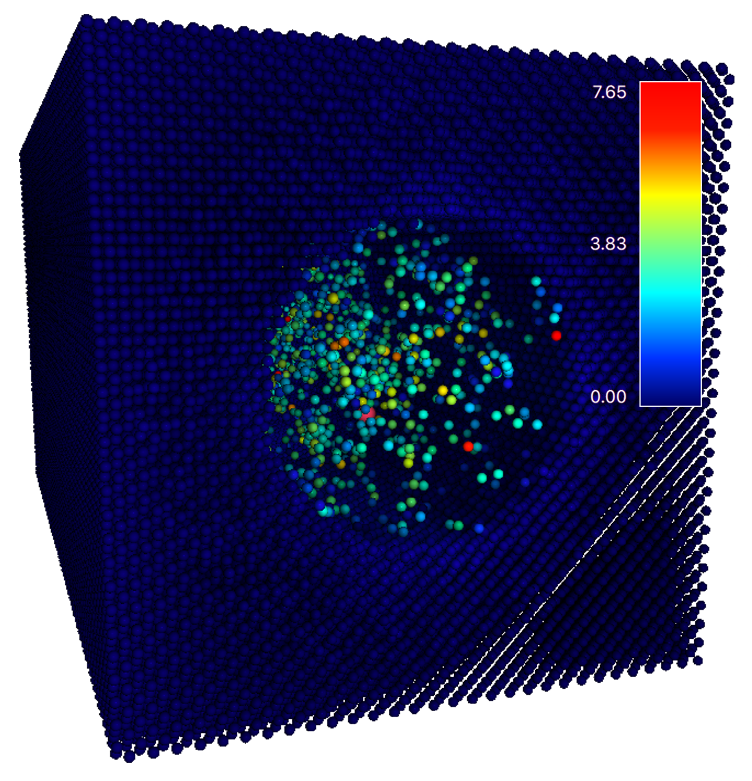
\includegraphics[width=0.8\textwidth]{lj_flow/07_moving.png}
	\caption{
		Snapshot of the system after $t=2.0$ where atoms are colored by their displacements since $t=0$.
		The outmost atoms are completely frozen as we see from the dark blue color meaning zero displacement.
		Atoms in the solid are also blue, but brighter, since they are thermally vibrating in the lattice.
		Inside the inner cylinder we see that the gas moves more freely since these atoms are not bounded.
	}
	\label{fig:moving_atoms}
\end{figure}

By rerunning again (\keys{Ctrl+R}), we confirm that the system behaves as expected as shown in figure \ref{fig:moving_atoms} where
atoms are colored based on their displacement.
The only remaining part now is to set up the commands that will apply the pressure gradient and measure the radial velocity profile.

\subsection{Pressure gradient and measurement}
To obtain a pressure gradient, we will apply a constant force in the positive $x$-direction on all the gas atoms.
A given pressure gradient must be specified. We will use $\nabla P = 0.001$, which was chosen so that it provides reasonable velocity profiles that demonstrate the wall slip effects.
In LAMMPS, we obtain this by adding the commands
%
\begin{lstlisting}
variable dP equal 0.001
variable force equal ${dP}/${rho_m}/0.5
fix flow gas addforce ${force} 0.0 0.0
\end{lstlisting}
%
To measure the velocity profile, we will use the built-in binning feature in LAMMPS called \textit{chunks},
a general concept where a \code{chunkID} is assigned to each atom
based on its position. LAMMPS supports multiple different \textit{chunk styles}, one of which is a cylinder.
In the cylinder binning, we choose the same properties as for a cylinder region (center, length etc.), but also the binsize in the length direction and how many radial bins we want.
We use one single bin in the flow direction since we only want to measure the radial velocity profile.
The command for giving each atom a \code{chunkID} is\footnote{The \& is used to continue the command on the next line since it is quite long.}
\begin{lstlisting}
compute chunk all chunk/atom bin/cylinder x lower &
$(lx) $c $c 0 $(v_R+3) 50 units box
\end{lstlisting}
This will create 50 radial bins for $r\in (0, R+3)$, where $R$ is the radius of the inner cylinder.
We measure in a cylinder that it slightly larger than the initially defined cylinder to see where the boundary is in the plot.
The final command we will use is the \code{fix ave/chunk} where we can get a smooth averaged velocity profile sampled over many timesteps
\begin{lstlisting}
fix vx all ave/chunk 10 10 100 chunk vx ave running
\end{lstlisting}
Here we use every 10th value to sample the velocity profile, keeping all samples to sum them into a larger histogram.
This fix will appear in the list of fixes in the \textit{Simulation} panel just as groups, regions, computes and variables.
When we click it, we will get the figure shown in figure \ref{fig:velocity_profile1}a.
\begin{figure}
	\centering
	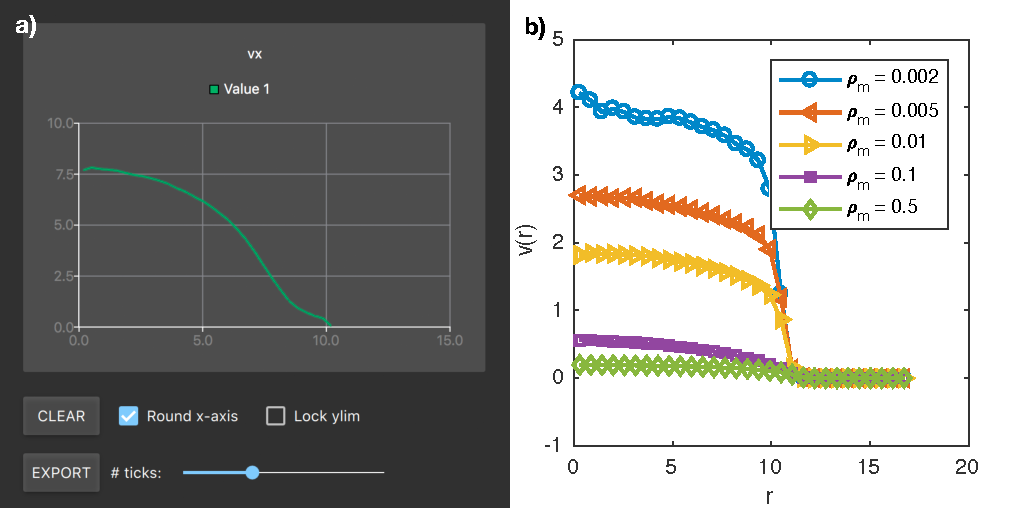
\includegraphics[width=\textwidth]{figures/velocity_profile.pdf}
	\caption{
		The velocity profile for a Lennard-Jones gas inside a nanochannel of radius 12.
		Atomify provides real-time plots as seen in a) and can export data to MATLAB, Python
		or raw text, which can be used to produce publication ready figures as in b).
		Here we have normalized the velocity profiles by the mean value so it is easier
		to compare the profile at different densities. The higher velocity near the boundaries at low densities
		is evident from these simulations.
	}
	\label{fig:velocity_profile1}
\end{figure}

\subsection{Results}
We conclude this case study with a series of simulations for different densities $\rho_m$.
Each simulation runs 5000 timesteps before starting to sample for another 50000 timesteps.
We export the plots from \code{fix vx} to MATLAB using the Export function seen in figure \ref{fig:velocity_profile1}a.
%
% It may be a good idea also to include the MATLAB script for completeness here
%
All these plots are now merged into a final figure which is shown in figure \ref{fig:velocity_profile1}b, where
we have normalized each velocity profile to its mean value so flow profiles are easier to compare.
The figure clearly demonstrates that the gases with lower density have a higher velocity near the boundary, which is an effect called plug flow.
As discussed before, what we observe here is the Klinkenberg effect, which explains why the permeability can be much higher for dilute gases than dense liquids.

\section{Availability}
Atomify is available on Linux and MacOS and can be downloaded from
\url{https://github.com/ovilab/atomify}
A lightweight version of Atomify is also available for mobile devices running
Android or iOS. This version runs LAMMPS on the device with real-time visualization
and supports simple interactions such as setting the temperature on thermostats.

\section{Acknowledgments}
This work is part of the Tight Rocks research program funded by Equinor ASA at the University of Oslo.

\section*{References}
\bibliography{Remote}
%
%\begin{thebibliography}{10}
%\bibitem{ref1} J.~Doe, Article name, \textit{Phys. Rev. Lett.}
%\bibitem{ref2} J.~Doe, J. Smith, Other article name, \textit{Phys. Rev. Lett.}
%\bibitem{web} \href{http://www.google.pl}{www.google.pl}
%\end{thebibliography}
\end{document}